\subsection{API}
Die API definiert einen Workflow der einen Service auf einer Cloud erstellt. Es ist offen, ob 
dieser Service über mehrere Cloud Anbieter hinaus geht. Der Service wird durch 
ein Konfigurationsfile definiert. Die Software auf den Instanzen wird durch Images installiert.
 Ein Service kann auch wieder gelöscht werden.
 Es ist nicht die Aufgabe der API existierende Services zu identifizieren. 
 Die API muss Modular sein, das heisst es sollte möglich sein andere oder eigene 
 Programme für die Cloud Kommunikation zu verwenden. Innerhalb der API 
 werden Compute, Storage, Network usw. als ServiceModule bezeichnet. 
 Diese Abstraktion ermöglicht das wiederverwenden und erweitern der API.
\newpage
\subsection{Customer-Dashboard}
\subsubsection{Homescreen}
Im Homescreen werden alle zu 
Verfügung stehenden Services angezeigt.
Hier werden die Services Offerings genannt um eine Unterscheidung zwischen 
Abonnierten Services (Services) und zur Verfügung stehenden Services (Offerings) 
machen zu können.
\newline
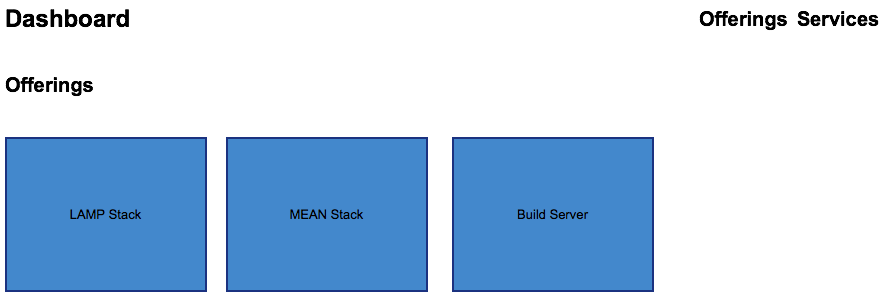
\includegraphics[width=\textwidth]{homescreen_customer}

\subsubsection{Services Übersicht}
In der Services Übersicht werden dem Customer alle abonnierten Services 
angezeigt und können hier auch gekündigt werden.
\newline
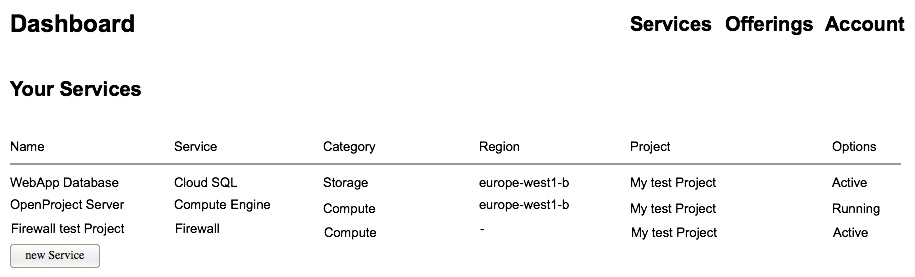
\includegraphics[width=\textwidth]{services_overview}


\subsubsection{Service abonnieren}
Sobald ein Service auf dem Homescreen ausgewählt wird und auf den ``subscribe'' 
Button geklickt wird, wird dieser abonniert und wird in der Services Übersicht 
angezeigt.
\newline

\includegraphics[width=\textwidth]{service_settings}


\newpage
\subsection{Admin-Dashboard}
Zusätzlich zum Customer-Dashboard soll ein Admin-Dashboard zur Verfügung stellen 
in welchem der Admin Services und Servicemodule erstellen kann.

\subsubsection{Service}
Ein Service hat einen bestimmten Namen und jedem Service sind eine gewisse 
Anzahl Servicemodule zugeteilt. um den Service abbilden zu können.
Hier kann der Admin den Service ändern und je nach Anforderung den Service 
anpassen.
\newline
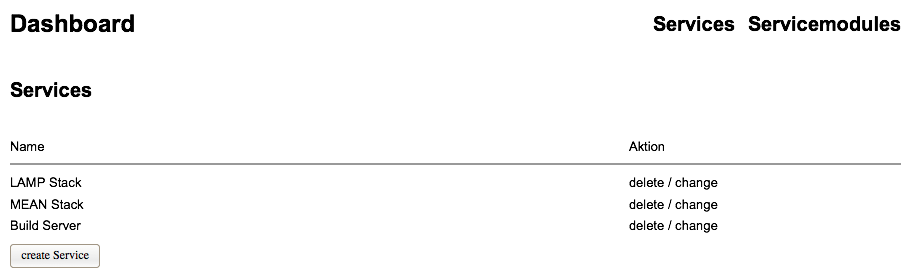
\includegraphics[width=\textwidth]{homescreen_admin}
